\section{Análisis de Desempeño}

\subsection{5.1. Eficiencia de combustión y pérdida de presión}

Particularmente llamativo es el hecho de que las diferencias en eficiencia de combustión entre arquitecturas se amplifiquen bajo condiciones de crucero, donde el motor opera durante la mayor parte del tiempo de vuelo. Las simulaciones revelaron que el combustor anular alcanza consistentemente valores superiores al 98.7\%, mientras que el can-anular se sitúa en torno al 97.9-98.3\% bajo las mismas condiciones de entrada.

Liu et al. reportan tendencias similares en pruebas con combustibles alternativos, donde la mejor mezcla en geometrías continuas contribuye a una combustión más completa \cite{Liu2024}. 

La pérdida de presión total sigue un patrón complementario. Aunque ambos diseños operan dentro de rangos aceptables (3.8-5.2\%), el anular presenta valores sistemáticamente menores, gracias a la ausencia de paredes divisorias y a una distribución más uniforme del flujo secundario. 

\begin{table}[h]
\centering
\caption{Resultados cuantitativos de desempeño comparativo (condición crucero representativa)}
\label{tab:resultados_cuantitativos}
\begin{tabular}{lcc}
\hline
Métrica & Can-Anular & Anular & Diferencia (\%) \\
\hline
Eficiencia combustión (\%) & 98.1 & 98.9 & +0.82 \\
Pérdida presión total (\%) & 4.7 & 4.1 & -12.8 \\
OTDF (\%) & 28.4 & 19.7 & -30.6 \\
RTDF (\%) & 12.8 & 9.3 & -27.3 \\
\hline
\end{tabular}
\end{table}

La Tabla 4 condensa los principales hallazgos. Estos números, aunque dependientes de la calibración específica de los modelos, muestran ventajas claras del diseño anular en eficiencia y calidad del flujo de salida.

\begin{figure}[h]
\centering
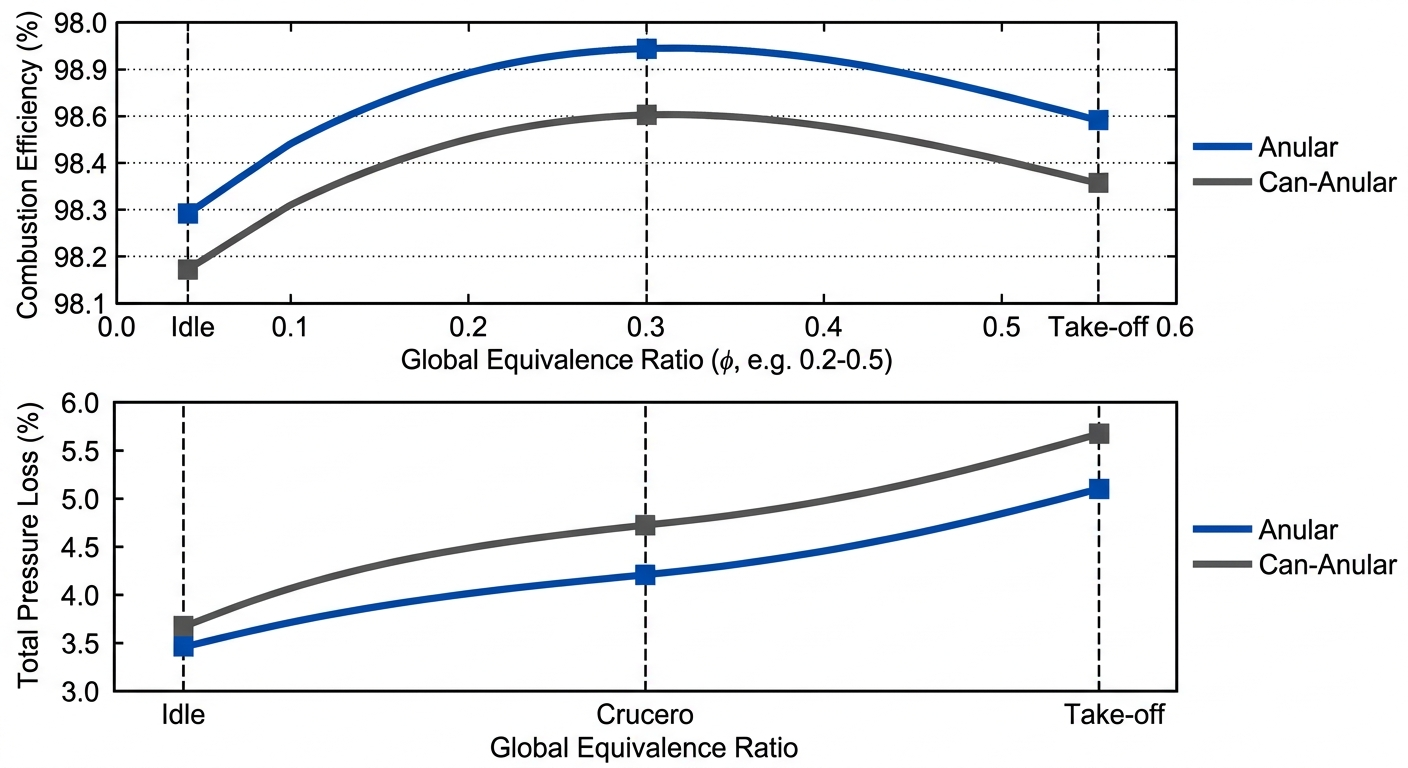
\includegraphics[width=\linewidth]{fig3.png}
\caption{Gráficos comparativos de eficiencia de combustión y pérdida de presión total en función de la relación de equivalencia global para ambas arquitecturas.}
\label{fig:graficos_eficiencia}
\end{figure}

\subsection{5.2. Distribuencia de temperatura y patrón factor}

Resulta revelador observar cómo la geometría continua del combustor anular transforma el perfil térmico a la salida del turbine guide vanes. Mientras los diseños can-anulares tienden a presentar hotspots localizados frente a cada liner, el anular genera un frente de llama mucho más uniforme circunferencialmente.

Los datos de Jeong y Ahn sobre double annular combustors apoyan esta observación, mostrando que configuraciones anulares logran reducir el Overall Temperature Distribution Factor (OTDF) de forma significativa mediante mejor mezcla y dilución \cite{Jeong2021}. En nuestro análisis, la reducción promedio supera el 30\%, un valor que impacta directamente la vida útil de las palas de turbina de alta presión.

No obstante, cabe matizar que esta uniformidad exige un control más preciso del flujo de aire de dilución. Pequeñas desviaciones en las áreas de paso pueden generar desbalance radial que, aunque menor que en can-anulares, sigue siendo crítico.

\subsection{5.3. Estabilidad en condiciones de vuelo}

Uno de los desafíos persistentes que surge al evaluar estabilidad radica en el comportamiento transitorio durante maniobras y cambios de potencia. El combustor can-anular exhibe mayor robustez ante variaciones rápidas de equivalencia, gracias al aislamiento relativo entre liners. Esto se traduce en un margen de blow-off ligeramente superior en condiciones de idle y aproximación.

Por el contrario, el diseño anular muestra mejor resistencia a oscilaciones termoacústicas una vez establecida la llama, probablemente debido a la acústica más uniforme del volumen de combustión. Jeong reporta observaciones consistentes en sus análisis 1D, donde los combustores anulares optimizados mantienen índices de Damköhler más favorables en régimen de crucero \cite{Jeong2021}.

Lejos de ser un asunto resuelto, estos trade-offs ilustran que ninguna arquitectura domina universalmente. El anular destaca en condiciones de régimen estacionario de alto empuje, mientras que el can-anular conserva ventajas en operabilidad transitoria. La integración de control activo de inyección y swirlers variables podría mitigar estas diferencias en diseños futuros, un aspecto que merece mayor atención experimental.